
\documentclass{article}

\usepackage{float}
\usepackage{textcomp}
\usepackage{polski}
\usepackage[utf8]{inputenc}
\usepackage[T1]{fontenc}
\usepackage{graphicx}
\graphicspath{ {res/} }



\usepackage[top=2cm, bottom=2cm, left=3cm, right=3cm]{geometry}

\makeatletter

\newcommand{\linia}{\rule{\linewidth}{0.5mm}}
\renewcommand\thesection{\arabic{section}}

\renewcommand{\maketitle}{\begin{titlepage}
		
		\vspace*{1cm}
		
		\begin{center}\small
			
			Politechnika Poznańska\\
			
			Wydział Elektryczny\\
			
			Kierunek Informatyka
			
		\end{center}
		
		\vspace{2cm}
		
		\linia
		
		\begin{center}
			
			\LARGE {\textbf{KakaduVoIP} \\[1cm]}
			\begin{figure}[h]
				\centering
				
\includegraphics[scale=0.2]{Kakadu}
			\end{figure}
		  \LARGE {Projekt zespołowy  \\ Telefonia IP}
			
		\end{center}
		
		\linia
		
		\vspace{3cm}
		
		\begin{flushright}
			
			\begin{minipage}{15cm}
				
				\textit{ \Large{Autorzy:}}\\
				
				\normalsize{\@author} \par
				
			\end{minipage}
			
		\end{flushright}
		
		\vspace*{\stretch{6}}
		
		\begin{center}
			
			\@date
			
		\end{center}
		
	\end{titlepage}%
	
}

\makeatother

\author{\Large{Szymon Zieliński \\[0.2cm] szymon.r.zielinski@gmail.com \\[0.2cm] 126812\\[0.4cm] Oskar Rutkowski \\[0.2cm] oskar.rutkowski@student.put.poznan.pl \\[0.2cm] 126845} }


\begin{document}
	
	\pagenumbering{gobble}
	\maketitle
	\newpage
	\tableofcontents
	\newpage
	\pagenumbering{arabic}
	
	\section{Charakterystyka ogólna projektu}
	\paragraph*{} Aplikacja pozwala na komunikowanie się użytkowników za pomocą mikrofonu oraz głośników w czasie rzeczywistym. Aplikacja jest stworzona w języku Java oraz działa w oparciu o architekturę klient-serwer. Użytkownik po uruchomieniu, jest proszony o podanie nazwy użytkownika oraz adresu serwera  do którego chce się połączyć. Będąc połączonym, użytkownik ma możliwość stworzenia własnego pokoju konferencyjnego lub dołączenia do istniejącego już pokoju. Aby połączyć się z pokojem wybranym z listy, użytkownik musi podać hasło pokoju. Po podaniu prawidłowego hasła, użytkownik ma możliwość rozmowy przy pomocy naciśniętego przycisku lub zmianę metody komunikacji na opcję mówienia ciągłego. Użytkownik ma możliwość wyciszenia swojego mikrofonu lub głośników, jak też innego użytkownika, znajdującego się w pokoju.
	\section{Architektura systemu}
	\paragraph*{} System KakaduVoIP jest oparty o model architektury klient-serwer. Model ten umożliwia podział zadań, serwer zapewnia usługi dla klientów, a klienci zgłaszają żądania obsługi. Serwer składuje informacje o pokojach w plikach lokalnych.
	\section{Wymagania}
	\paragraph*{} W tym paragrafie zostaną omówione wymagania aplikacji funkcjonalne oraz niefunkcjonalne.
	\subsection{Wymagania funkcjonalne}
	\begin{itemize}
		\item użytkownik łączy się z systemem jedynie za pomocą nazwy użytkownika oraz adresu serwera,
		\item użytkownik może zmieniać ustawienia aplikacji względem możliwości komunikowania się, tj. mówienie przez naciśnięcie przycisku lub mówienie ciągłe,
		\item użytkownik może utworzyć pokój konferencyjny, nadając mu nazwę i hasło dostępu do pokoju oraz tworząc hasło administracyjne, stając się administratorem tego pokoju,
		\item administrator pokoju, który stworzył pokój, może usunąć pokój konferencyjny,
		\item administrator, który założył pokój, może wyrzucić innych użytkowników z pokoju.
		\item użytkownik może dołączyć do pokoju wybranego z listy aktualnie dostępnych pokoi na serwerze, podając hasło dostępu do pokoju,
		\item użytkownik w pokoju konferencyjnym może opuścić pokój,
		\item użytkownik w pokoju konferencyjnym może wyciszyć innego użytkownika, aby go nie słyszeć,
		\item użytkownik w pokoju konferencyjnym może komunikować się z innymi użytkownikami za pomocą przycisku lub mówienia ciągłego,
		\item użytkownik w pokoju konferencyjnym może wyciszyć swój mikrofon lub wyłączyć używanie głośników,
		
	\end{itemize}
	\subsection{Wymagania niefunkcjonalne}
	\begin{itemize}
		\item nowo utworzony pokój nie potrzebuje administratora pokoju będącego aktualnie w pokoju,
		\item pokój może być usunięty przez administratora pokoju dzięki podaniu hasła dostępu do pokoju oraz hasła administracyjnego,
		\item po usunięciu pokoju przez administratora pokoju, wszyscy użytkownicy zostają automatycznie przekierowani do głównej strony aplikacji,
		\item aplikacja klienta oraz serwer napisane w języku Java,
		\item aplikacja wieloplatformowa,
		\item szyfrowanie dźwięku,
		\item szyfrowanie zapytań do serwera,
		\item do połączenia z serwerem nie jest potrzebna rejestracja użytkownika, jedynym wymogiem jest podanie nazwy użytkownika oraz adres serwera,
		\item do składowania haseł zabezpieczających pokoje, posłużą pliki lokalne składowane na serwerze,
		\item hasła dostępu do pokoju oraz hasła administracyjne będą poddane funkcji haszującej,
		\item interfejs stworzony w języku polskim,
		\item do sprawnego działania aplikacji, niezbędne są słuchawki lub głośniki oraz mikrofon.
	\end{itemize}
	\section{Narzędzia, środowiska, biblioteki, kodeki}
	\paragraph*{} W niniejszym paragrafie zostaną opisane wykorzystane w aplikacji narzędzia, środowiska, biblioteki oraz kodeki.
	\paragraph*{} Głównym językiem wykorzystanym do napisania aplikacji jest język Java w wersji 8 Update 162. Wykorzystana jest technika Maven Project, dzięki której możliwa jest praca w różnych środowiskach programistycznych takich jak Intellij oraz Eclipse Oxygen.
	\paragraph*{} Wykorzystane frameworki oraz biblioteki:
	\begin{itemize}
		\item Apache MINA - Open Source Framework, służący do budowania aplikacji sieciowych,
		\item Java Media Framework - technologia umożliwiająca wstawianie multimediów do aplikacji napisanych w języku Java oraz transmisję audio za pomocą protokołu RTP,
		\item Protocol Buffers - narzędzie do tworzenia własnych protokołów,
		\item java.security.MessageDigest - biblioteka wykorzystana do nakładania funkcji skrótu na hasła,
		\item javax.security oraz javax.crypto - biblioteki wykorzystane do szyfrowania.
	\end{itemize}
	\paragraph*{} Hasła wraz z potrzebnymi informacjami o pokojach oraz użytkownikach są przetrzymywane w plikach lokalnych przechowywanych po stronie serwera.
	\paragraph*{} Użyte kodeki, zawarte w JMF:\\ MPEG Layer II Audio (.mp2) [MPEG layer 2 audio ]
	\section{Protokoły}
	\paragraph*{} Jednymi z najważniejszych protokołów użytych są:
	\begin{itemize}
		\item Warstwa aplikacji:
		\begin{itemize}
			\item RTP - protokół transmisji w czasie rzeczywistym - do przesyłania dźwięku,
			\item RTCP (ang. Real Time Control Protocol) - protokół sterujący używany do okresowej transmisji pakietów kontrolnych do wszystkich uczestników sesji. Pozwala monitorować dostarczanie danych przez protokół RTP i transport zwrotnej informacji odnośnie jakości transmisji,
			\item protokoły własne - protokoły do komunikacji z serwerem:
			\begin{enumerate}
				\item protokół do połączenia z serwerem,
				\item protokół do przesłania listy dostępnych pokoi,
				\item protokół do zarządzania pokojami(tworzenie, usuwanie),
				\item protokół służący do dołączania/wychodzenia z pokoju,
				\item protokół pozwalający na wyciszenie innego użytkownika. 
			\end{enumerate}
		\end{itemize}
		\item Warstwa transportowa:
		\begin{itemize}
			\item TCP - protokół kontroli transmisji - do komunikacji z serwerem,
			\item UDP - transportowy protokół bezpołączeniowy - do przesyłania próbek z dźwiękiem.
		\end{itemize}
		\item Warstwa sieci:
		\begin{itemize}
			\item IP - podstawowy protokół stosowany w Internecie.
		\end{itemize}
	\end{itemize}
	\section{Schemat bazy danych} 
	\paragraph{} W niniejszym paragrafie zostanie przedstawiony schemat bazy przechowującej dane pokojów.
	\begin{figure}[h]
		\centering
		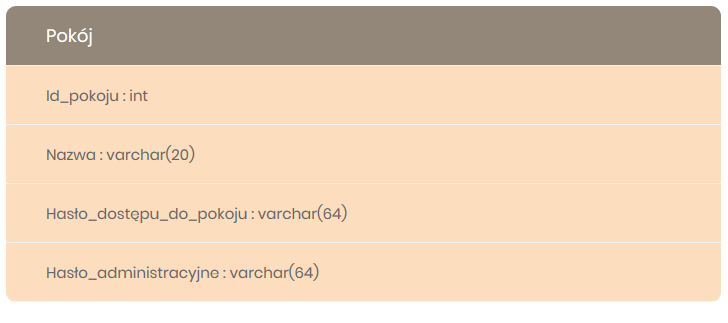
\includegraphics[scale=0.7]{BD}
		\caption[]{Model tabeli Pokój}
		\label{fig:BD}
	\end{figure}

	Zgodnie z rysunkiem \ref{fig:BD}, baza danych składa się z jednej tabeli opisującej pokój. Id\_pokoju wskazuje na identyfikator konkretnego utworzonego przez użytkownika pokoju. Nazwę pokoju nadaje użytkownik podczas tworzenia pokoju. Hasło dostępu do pokoju oraz hasło administracyjne są wynikiem funkcji skrótu. 
	\section{Diagramy UML}
	\subsection{Diagramy przypadków użycia}
	\paragraph{} W niniejszym paragrafie zostanią przedstawione diagramy UML aktorów oraz ich zadań funkcjonalnych.
	\begin{figure}[H]
		\centering
		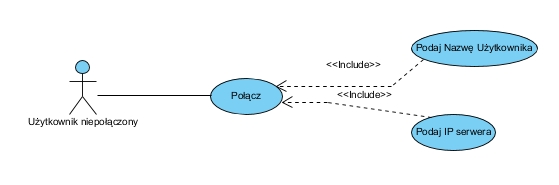
\includegraphics[scale=0.9]{UserNP}
		\caption[]{Diagram użytkownika niepołączonego}
		\label{fig:DUN}
	\end{figure}
	\begin{figure}[H]
		\centering
		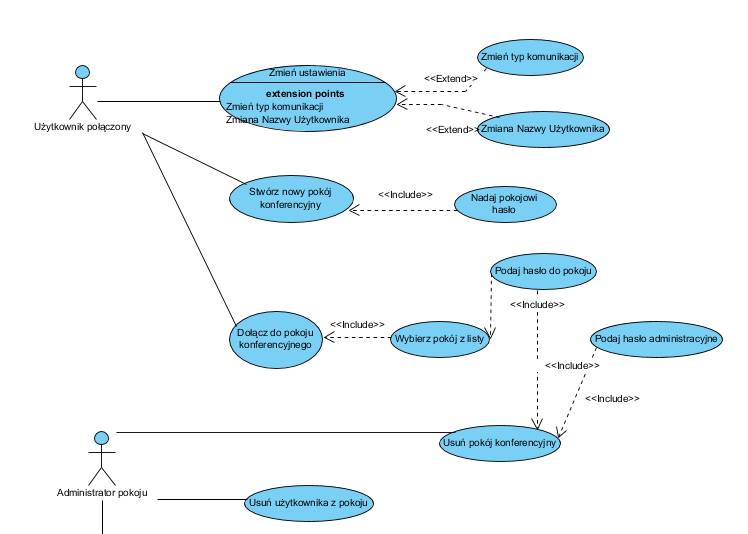
\includegraphics[scale=0.9]{UserPiAdm}
		\caption[]{Diagram użytkownika połączonego oraz administratora pokoju}
		\label{fig:DUP}
	\end{figure}
	\begin{figure}[H]
		\centering
		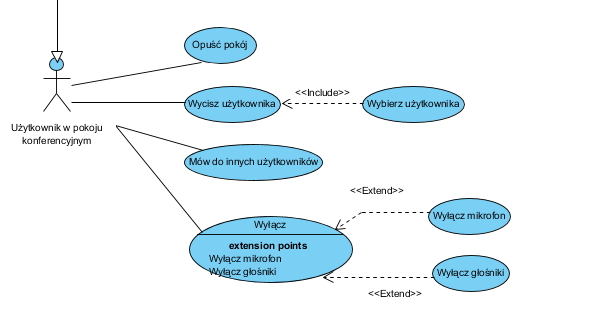
\includegraphics[scale=0.9]{UserPK}
		\caption[]{Diagram użytkownika w pokoju konferencyjnym}
		\label{fig:DUW}
	\end{figure}
	\subsection{Diagramy sekwencji}
	\paragraph{} W niniejszym paragrafie zostanią przedstawione diagramy UML przedstawiające proces łączenia się użytkownika z serwerem, tworzenia pokoju konferencyjnego oraz usuwania pokoju konferencyjnego.
	\begin{figure}[H]
		\centering
		\hspace*{-2cm} 
		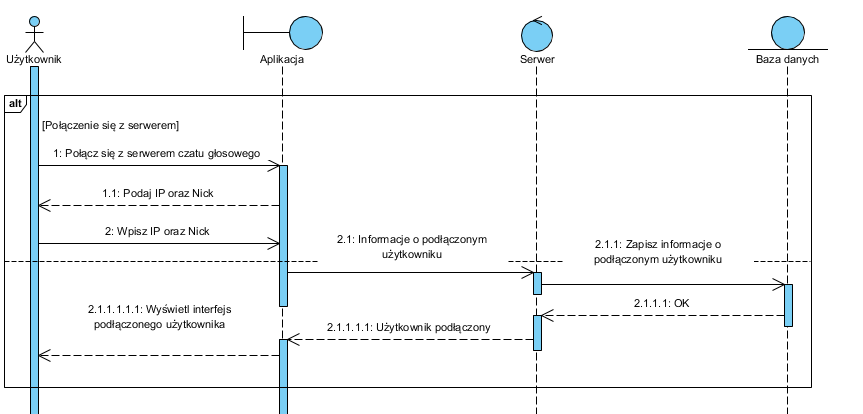
\includegraphics[scale=0.9]{seq1}
		\caption[]{Diagram połączenia z serwerem}
		\label{fig:seq1}
	\end{figure}
	\begin{figure}[H]
		\centering
		\hspace*{-2cm} 
		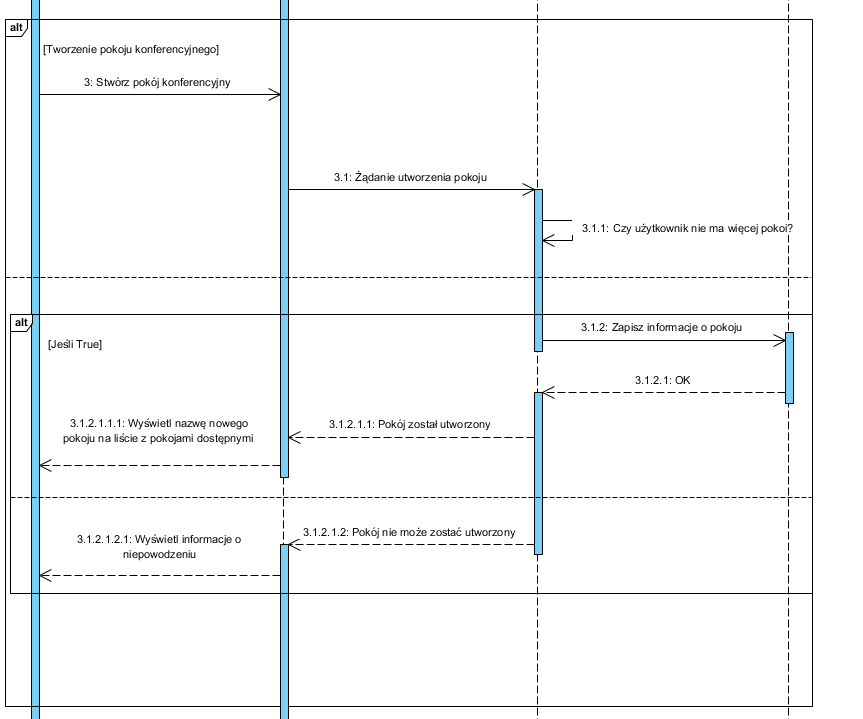
\includegraphics[scale=0.9]{seq2}
		\caption[]{Diagram tworzenia pokoju konferencyjnego}
		\label{fig:seq2}
	\end{figure}
	\begin{figure}[H]
		\centering
		\hspace*{-2cm} 
		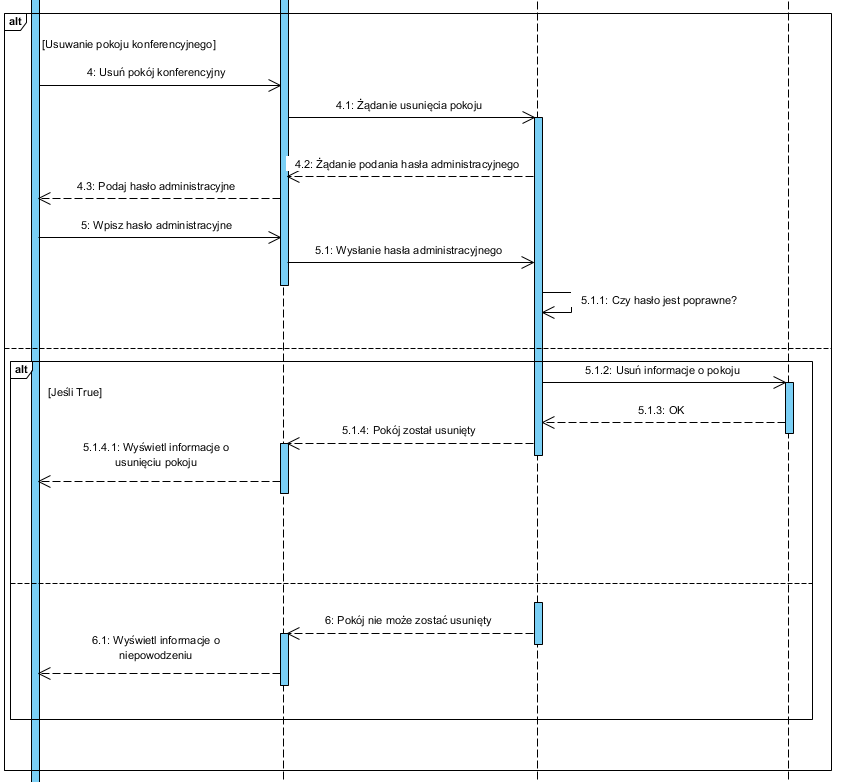
\includegraphics[scale=0.9]{seq3}
		\caption[]{Diagram usuwania pokoju konferencyjnego}
		\label{fig:seq3}
	\end{figure}
	\section{Projekt interfejsu graficznego}
	\paragraph*{} W paragrafie zostanie przedstawiony projekt interfejsu graficznego aplikacji.
	\begin{figure}[H]
		\centering
		\hspace*{0cm} 
		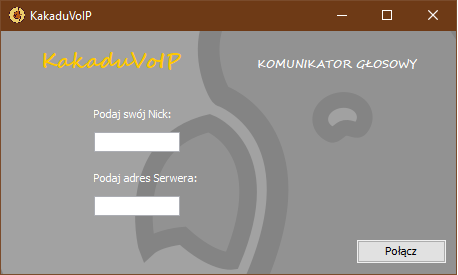
\includegraphics[scale=0.9]{glowna}
		\caption[]{Interfejs ekranu połączenia}
		\label{fig:gui1}
	\end{figure}
	\begin{figure}[H]
		\centering
		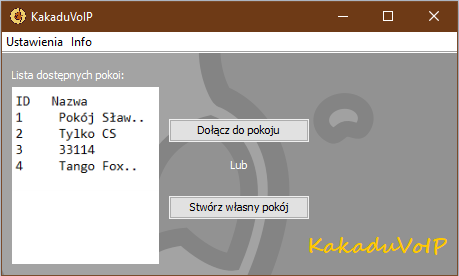
\includegraphics[scale=0.9]{glowna2}
		\caption[]{Interfejs ekranu głównego aplikacji}
		\label{fig:gui2}
	\end{figure}

\end{document}